\chapter{Hardware}

As we said before, the hardware includes the physical parts of a computer that \textbf{can be physically touched}. Those different components have a different function that we will detail later.

It is possible that we already know some of these components, but we must know the origin and how the architecture of modern computers arises.

\section{Von Neumann architecture}

The first electromechanical computers were designed for a single purpose, they were "designed" to perform a task. A known case might be \href{https://en.wikipedia.org/wiki/Bombe}{\textbf{Bombe}}, an electromechanical machine capable of cracking Nazi Enigma crypto systems. \movie{https://www.imdb.com/title/tt2084970/}{The Imitation Game}

Some of those computers could be "reprogrammed", but based on rewiring different components after a study of what the “operators” (the persons that operate the machine) wanted. It could take up to three weeks to prepare an ENIAC program and get it working.

The concept of universal computing machines and the use of stored programs already existed on a theoretical level since the mid-1930s (written by \href{https://es.wikipedia.org/wiki/Alan_Turing}{Alan Turing}).

The mathematician and physicist \href{https://es.wikipedia.org/wiki/John_von_Neumann}{John von Neumann}, along with other colleagues, \textbf{describes in 1945 a design for a computer architecture} in which describe the following components that interrelate with each other through the system bus that acts as a communication channel between them:

\vspace{-10pt}
\begin{center}
    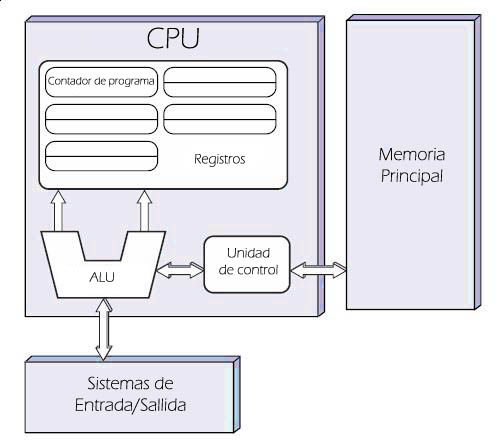
\includegraphics[width=0.5\linewidth]{vonneumann.jpg}
    \captionof{figure}{Von Neumann Architecture. Source: \href{https://es.wikipedia.org/wiki/Arquitectura_de_Von_Neumann}{wikipedia}}
\end{center}

\begin{itemize}
    \item \textbf{Central Processing Unit} (\textbf{CPU}), which contains:
    \begin{itemize}
        \item \textbf{Arithmetic Logic Unit} (\textbf{ALU}): It is a digital circuit that performs arithmetic operations (addition, subtraction, multiplications,...) and logic operations (AND, OR, X-OR, ...) between the values of the arguments (one or two).

        \item \textbf{Processor Registers}: High-speed, small-capacity memory built into the CPU to store data used during program execution. For example:
        \begin{itemize}
            \item Program Counter (\textbf{PC})
            \item Accumulator
            \item Instruction Register (\textbf{IR})
        \end{itemize}
        \item \textbf{Control unit}: Its function is to search for instructions in main memory, decode them and execute them, using the processing unit for this.
    \end{itemize}
    \item The \textbf{main memory}: System where the instructions and data of the program that is being executed at that moment are stored. The memory is divided into cells that are identified by a single address.

    \item \textbf{Buses}: The path through which instructions and data flow between the different computer units.

    \item The \textbf{Input/Output systems}: Used to transfer  information between input and/or output peripherals to extend the capabilities of the equipment.
\end{itemize}

It is more complex, there are more registers, more instructions, ... but the idea is the same

\infobox{\textbf{We can see a simulation of the Von Neumann Architecture \href{https://lab.xitrus.es/VonNeumann/}{here}}}



\section{CPU}

The CPUs are classified by the set of instructions it can interpret. There are some set of instructions, but the more used are:

\begin{itemize}
    \item “\textbf{Complex Instruction Set Computer}”: \textbf{CISC}. Is a computer architecture in which single instructions can execute several low-level operations (such as a load from memory, an arithmetic operation, and a memory store. Has many specialized instructions, some of which may only be rarely used in practical programs. For example: Intel's \textbf{x86}.

    \item “\textbf{Reduced Instruction Set Computer}”: \textbf{RISC}. Is a computer designed to simplify the individual instructions given to the computer to accomplish tasks. For example: IBM's PowerPC, \textbf{ARM} (Qualcomm Snapdragon, Apple's iPhones and M1).
\end{itemize}

\begin{yukitblrcol}{colspec={X[1]X[2]X[2]},measure=vbox}
    & CISC & RISC \\
    Advantages & \begin{itemize}
            \item The compiler requires little effort to translate programs.
            \item Requires fewer configured instructions than RISC.
        \end{itemize}
       &
         \begin{itemize}
             \item 1 instruction, 1 clock cycle.
             \item They allow to reduce the execution times of a process
             \item More efficient: requires less power consumption and generates less heat than RISC processors.
         \end{itemize} \\
    Disadvantage &
        \begin{itemize}
            \item May require multiple clock cycles to complete a software instruction.
            \item The performance of the computer suffers a decrease due to the speed of the clock.
            \item They have a much larger design than RISC architecture, which leads to more heat generation, higher power consumption and higher physical space requirement.
        \end{itemize}
     &
        \begin{itemize}
            \item Processor performance may vary depending on the code being executed.
            \item Most software and compilers make use of complex instructions.
        \end{itemize}
     \\
\end{yukitblrcol}


%\section{Motherboard}
%
%
%\subsection{Socket}




%\section{RAM}
%
%\section{Storage}
%
%\subsection{Hard Disks}

%\section{Power supply}